\documentclass[sigconf,natbib=false]{acmart}
%%
%% \BibTeX command to typeset BibTeX logo in the docs
\AtBeginDocument{%
  \providecommand\BibTeX{{%
    \normalfont B\kern-0.5em{\scshape i\kern-0.25em b}\kern-0.8em\TeX}}}

%% Rights management information.  This information is sent to you
%% when you complete the rights form.  These commands have SAMPLE
%% values in them; it is your responsibility as an author to replace
%% the commands and values with those provided to you when you
%% complete the rights form.
\setcopyright{acmlicensed}
\copyrightyear{2025}
\acmYear{2025}
\acmDOI{XXXXXXX.XXXXXXX}

%% These commands are for a PROCEEDINGS abstract or paper.
\acmConference[ACM REP'25]{2025 ACM Conference on Reproducibility and Replicability}{July 29-31, 2025}{Vancouver, Canada}
%
%  Uncomment \acmBooktitle if th title of the proceedings is different
%  from ``Proceedings of ...''!
%
%\acmBooktitle{Woodstock '18: ACM Symposium on Neural Gaze Detection,
%  June 03--05, 2018, Woodstock, NY} 
\acmISBN{978-1-4503-XXXX-X/18/06}

\usepackage{tcolorbox}
\tcbuselibrary{theorems}
\usepackage{cleveref}
\newtcbtheorem[]{trap}{Pitfall}{colback=black!5,colframe=black!35,fonttitle=\bfseries}{th}
\newtcbtheorem[]{lesson}{Takeaway}{colback=black!5,colframe=black!35,fonttitle=\bfseries}{th}
\newcommand{\repro}{reproducibility}
\newcommand{\Repro}{Reproducibility}
\newcommand{\transpo}{\emph{Transposition}}
\newcommand{\flavour}{\emph{flavour}}
\newcommand{\flavours}{\emph{flavours}}
\newcommand{\ie}{\emph{i.e.,}}
\newcommand{\eg}{\emph{e.g.,}}
\newcommand{\nix}{\emph{Nix}}
\newcommand{\nixos}{\emph{NixOS}}
\newcommand{\nxc}{\emph{NixOS Compose}}
\newcommand{\enos}{\emph{EnOSlib}}
\newcommand{\grid}{\emph{Grid'5000}}
\newcommand{\kam}{\emph{Kameleon}}
\newcommand{\kad}{\emph{Kadeploy}}
\newcommand{\mel}{\emph{Melissa}}
\newcommand{\store}{\emph{Nix Store}}
\newcommand{\ad}{Artifact Description}
\newcommand{\aeval}{Artifact Evaluation}
\newcommand{\adae}{\ad/\aeval}
\newcommand{\df}{\texttt{Dockerfile}}
\newcommand{\ecg}{\texttt{ecg}}
\newcommand{\todo}[1]{{\color{red}{TODO: #1}}}
\usepackage{hyperref}
\usepackage{array}
\usepackage{caption}
\usepackage{subcaption}
\usepackage{graphicx}
\usepackage{siunitx}
%\usepackage[table]{xcolor}
\usepackage{multirow}
\usepackage{hhline}
\usepackage{calc}
%\usepackage{tabularx}
\usepackage{fontawesome}
\usepackage[para,online,flushleft]{threeparttable}
\usepackage{booktabs}
\usepackage{longtable}
\usepackage{amsmath,amsfonts}
\usepackage{textcomp}
\usepackage[inline]{enumitem}  % enhanced enumerations
\usepackage{listings}
\definecolor{commentcolour}{rgb}{0.04,0.43,0.17}
\definecolor{keywordcolour}{rgb}{0.65,0.15,0.64}
\definecolor{backcolour}{rgb}{1,1,1}
\definecolor{linenumbercolour}{rgb}{0.1,0.1,0.1}
\definecolor{stringcolour}{rgb}{0.56,0.06,0.49}
\lstdefinestyle{mystyle}{
  backgroundcolor=\color{backcolour},   
  commentstyle=\color{commentcolour},
  keywordstyle=\color{keywordcolour},
  numberstyle=\tiny\color{linenumbercolour},
  stringstyle=\color{stringcolour},
  basicstyle=\ttfamily\footnotesize,
  breakatwhitespace=false,         
  breaklines=true,                 
  captionpos=b,                    
  keepspaces=true,                 
  numbers=left,                    
  numbersep=5pt,                  
  showspaces=false,                
  showstringspaces=false,
  showtabs=false,                  
  tabsize=2,
  framexrightmargin=-12pt
}
\lstset{style=mystyle, frame=single}

%\usepackage[backend=biber,style=trad-abbrv,firstinits=true]{biblatex}
\usepackage[
  datamodel=software,
  style=trad-abbrv,
  backend=biber
]{biblatex}
\addbibresource{references.bib}
\usepackage{software-biblatex}

\begin{document}

\title{%
  % (Very) Preliminary Study of the Longevity of Docker Images from Research Artifacts
  Longitudinal Study of the Software Environment Produced by Dockerfiles from Research Artifacts: Initial Design and Results
}

\author{Quentin Guilloteau}
\email{quentin.guilloteau@inria.fr}
\affiliation{%
  \institution{INRIA}
  \country{France}
}

% \renewcommand{\shortauthors}{Trovato and Tobin, et al.}

%%
%% The abstract is a short summary of the work to be presented in the
%% article.
\begin{abstract}
  The reproducibility crisis struck all the fields of Science, including Computer Science.
  To tackle the issue, the CS community set up artifact evaluation processes in conferences and journals to evaluate the reproducibility of the results shared in the publications.
  Authors thus share their artifacts included code, data and software environment required to reproduce the results.
  One method for sharing the software environment, that has been ``advertised'' by conferences and journals, is to use container technologies such a Docker and Apptainer.
  However, these tools relies on non-reproducible tools, hence producing non-reproducibile containers.

  In this paper, we present a tool and methodology to evaluate the variation in software environments through time of container images from research artifacts.
  We also present initial results on a small set of \df s from the EuroPar'24 conference.
\end{abstract}

%% %% The code below is generated by the tool at http://dl.acm.org/ccs.cfm.
%% Please copy and paste the code instead of the example below.
%%
\begin{CCSXML}
<ccs2012>
 <concept>
  <concept_id>00000000.0000000.0000000</concept_id>
  <concept_desc>Do Not Use This Code, Generate the Correct Terms for Your Paper</concept_desc>
  <concept_significance>500</concept_significance>
 </concept>
 <concept>
  <concept_id>00000000.00000000.00000000</concept_id>
  <concept_desc>Do Not Use This Code, Generate the Correct Terms for Your Paper</concept_desc>
  <concept_significance>300</concept_significance>
 </concept>
 <concept>
  <concept_id>00000000.00000000.00000000</concept_id>
  <concept_desc>Do Not Use This Code, Generate the Correct Terms for Your Paper</concept_desc>
  <concept_significance>100</concept_significance>
 </concept>
 <concept>
  <concept_id>00000000.00000000.00000000</concept_id>
  <concept_desc>Do Not Use This Code, Generate the Correct Terms for Your Paper</concept_desc>
  <concept_significance>100</concept_significance>
 </concept>
</ccs2012>
\end{CCSXML}

\ccsdesc[500]{Do Not Use This Code~Generate the Correct Terms for Your Paper}
\ccsdesc[300]{Do Not Use This Code~Generate the Correct Terms for Your Paper}
\ccsdesc{Do Not Use This Code~Generate the Correct Terms for Your Paper}
\ccsdesc[100]{Do Not Use This Code~Generate the Correct Terms for Your Paper}

%%
%% Keywords. The author(s) should pick words that accurately describe
%% the work being presented. Separate the keywords with commas.
\keywords{Reproducibility, Artifact Evaluation, Badges, Lifetime}

\received{12 February 2024}
\received[revised]{12 March 2009}
\received[accepted]{5 June 2009}

%%
%% This command processes the author and affiliation and title
%% information and builds the first part of the formatted document.
\maketitle

%% PAPER STARTS HERE -----------------------------------------------------------------------------------------------

\section{Introduction}

% \todo{split into intro and related work?}
% 
% \begin{itemize}
% \item Reproducibility crisis \cite{baker500ScientistsLift2016}
% \item Also in computer science \cite{collberg_repeatability_2015}, but most impact is from the missing environment.
% \item Artifact evaluation in conferences \cite{kidwell2016badges}
% \item Software environment is a problem/difficul aspect \cite{mytkowicz_producing_nodate}
% \item conferences recommand to use containers to share the software environmnent,
% \item more and more papers are linking code \cite{paperswithcode, kang2023papers, hong2013software}
% \item a lot of papers proposing solution around virtualisation and container \cite{brammer2011paper, brinckman2019computing}
% \item but container recipes are based on non-reproducibile tools (package managers and bad practices) \cite{guilloteau2024longevity, guilloteau2024frustrations}
% \item even though Nix \cite{dolstra_nix_2004} and Guix \cite{courtes_functional_2013} already very good solutions but not used enough \cite{guilloteau2024longevity}
% \item trade-off between storing the result of the image builts by the authors and the recipe \cite{software_heritage_2017, zenodo, figshare}
% \item we need the dev environment to \emph{inspect} and introduce \emph{variation} \cite{mercier2018considering}. \cite{blinry, nvidia_cuda_lifetime}
% \end{itemize}

The entire scientific community has been struck by the ``Reproducibility Crisis''~\cite{baker500ScientistsLift2016}, and Computer Science does not make exception~\cite{collberg_repeatability_2015}.
In order to improve the reproducibility of articles in Computer Science, the community set up \adae\ processes~\cite{kidwell2016badges} where authors would submit (if they want) the artifact required to reproduced the main results from their article.
Then a set of artifact reviewers would try to reproduce those main results given the artifact from the authors.
Based on the result of the reproduction attempt, the article is then awarded \emph{badges} to promote its reproducibility aspect.
The link to the artifacts can be found in the published version of the article, sometimes with an appendix giving more information about the artifact (\eg\ download instructions, hardware requirements, experiments workflow) \cite{paperswithcode, kang2023papers, hong2013software}.

One difficult aspect of creating a truly reproducible artifact is to properly control the software environment: packages and libraries versions.
Several works already shed light on the possible varability of results given a badly captured software environment \cite{mytkowicz_producing_nodate} \todo{more}.
To tackle this issue, the conference \ae\ committees have been pushing the authors to provide containers or virtual machines to share their artifacts in order to ``freeze'' their software environment.
However, authors generate their artifact right before the artifact submission~\cite{guilloteau2024longevity, guilloteau2024frustrations}.
Moreover, in the case of usual virtualisation techiniques to generate containers or virtual machines, users have to write the recipe made of a list of commands to execute from a base image.
This approach has several limitations.
First, these base images can vary, either because of bad practices from the users (\eg\ using the \texttt{latest} version of the images) or from the administrators of the image (\eg\ pushing a different image to a previously defined tag).
These base images can also be removed by the administrators making all the recipes unbuildable~\cite{nvidia_cuda_lifetime}.
Another limitation of this approach is the heavy dependency on non-reproducible tools such as classical package managers (\eg\ \texttt{apt}, \texttt{dpkg}, \texttt{yum}).
Hence, rebuilding a recipe of a container or a virtual machine can yield different results, and thus ``breaking'' the reproducibility of the results.
One solution would be to store the container itself (\ie\ the tarball) onto some long term storage for example Zenodo~\cite{zenodo}.
But this come with the downside of requiring more storage space than just storing the recipe (binary vs. text file).
This practice has thus some \textbf{severe scalability issues in terms of longevity}.
Moreover, storing the built binary image exhibits limitations when needed to \emph{inspect} the actual content of the image, and when a modification of the software environment capture by this image is needed~\cite{mercier2018considering}.
Having the opportunity to extend previous scientific work \todo{...}

A better solution would be to use tools such as Nix~\cite{dolstra_nix_2004} or Guix~\cite{courtes_functional_2013} which are focused on reproducibility and which are able to rebuild the \emph{exact same} software environment from a textual description and with longevity properties~\cite{courtes2024source}, but these tools are unfortunately poorly adopted by the community~\cite{guilloteau2024longevity}.


In this paper, we propose our \textbf{inital design of a longitudinal study of the variations through time of the software environment produced by \df s from research artifacts.}
We show initial results from five \df s extracted from the EuroPar'24 conference reproducibility artifacts built every month for six months.
\todo{The goal is not to dunk on authors or conferences, but simply to exhibit the potential issues with \df s.}

% We aim to answer the following questions:
% 
% \begin{enumerate}
% \item How does the packages evolve through time when captured in a \texttt{Dockerfile}?
% \item Which packaging tool is the most victim to variation in its resulting software environment?
% \item Which are the most volatile packages?
% \item Which practices in \df s are the most damaging to reproducibility?
% \end{enumerate}



% \newpage
\section{The \ecg\ Framework}

%% \begin{itemize}
%% \item `ecg`, Python tool, Licence, lines of code
%% \item architecture (nickel, what is supported)
%% \item process (submit new artifacts)
%% \item end goal of the project
%% \end{itemize}                   

In this section, we present \ecg, a tool for the periodic building of \df s from research artifacts and the collection of software environment informations.
\ecg\ is a 280-line Python3 script under the GPLv3 licence.

\subsection{Artifact representation}

An \df\ from an artifact is represented as a Nickel~\cite{nickel} file.
Nickel is a configuration language with functional paradigm.
One of it's feature is the possibility go ``verify'' that an configuration is ``well-formed'' with a \emph{contract}.
This Nickel file is then \emph{verified} against the contract (\todo{link to contract}) and translated to a JSON file fed to \ecg.

\begin{lstlisting}[caption=Example of Artifact representation in the Nickel format.]
{
  version = "1.0",
  artifact_url = "https://zenodo.org/.../artifact.zip",
  type = "zip",
  doi = "10.5281/zenodo.XXXXXXXX",
  conf_date = 2024,
  virtualization = "docker",
  buildfile_dir = "artifact",
  package_managers = [ "dpkg", "pip" ]
  git_packages = [
    { name = "spack", location = "/home/user/spack" }
  ],
  misc_packages = [
    {
      name = "cmake-3.22.2-linux",
      url = "https://github.com/Kitware/CMake/releases/download/v3.22.2/cmake-3.22.2-linux-x86_64.sh"
    }
  ]
}
\end{lstlisting}


\subsection{What do we capture?}

\subsubsection{Hash of the Artifact}

The articles give the link to the artifact.
This artifact can be shared in several ways, but not all ways have the same guarantees in terms of longevity and ``stability'' of the link.
Hence, we capture the result of the download at the given link (success or error).
In case of a succesful download, we also compute the cryptographic hash of the result of download to capture any variation in the source of the artifact which could explain later variations in the resulting software environment.

For instance, authors can give the link to a Zenodo archive that will \emph{always} point to the latest version of an artifact.
Hence, the content of the artifact behind this link can change through time.

\subsubsection{Docker Building Error}

In the case of a \df s failing to build, we capture the error (missing image, failing command, etc.).
In fact, we are only able to capture the first error of the build even if there might be several errors in the building process.
The Docker error is extracting by \texttt{grep}ing the building process log.

\subsubsection{List of Installed Packages and their Version}

The software environment can be composed of several packages.
Theses packages can have been installed by different means.
The most common way is through package managers (\eg\ \texttt{apt}, \texttt{dpkg}, \texttt{yum}).
But there are also installed packages for programming languages such as with \texttt{pip} for Python.
Another way to install package is to download the sources and build them locally.
\ecg\ is able to capture these different ways to install packages.
Hence, for each package, we extract the package name, the version (the \texttt{git} commit if using \texttt{git}), and the tool used to install the package.

As of for now, \ecg\ is able to query information from popular package managers (\texttt{dkpg} (and thus \texttt{apt}), \texttt{pacman}, \texttt{pip}, \texttt{conda}) and to deal with situations where packages are install by source (\texttt{package\_manager} in Listing 1).
In the case where there is a \texttt{git clone} command in the \df\ (\texttt{git\_packages} in Listing 1), \ecg\ will extract the commit of the local clone of the repository after the successful build of the container.
This allows us to trace the version of the package.
In the case of a simple downloading of the sources of a package (\texttt{misc\_packages} in Listing 1), for example with \texttt{wget} or \texttt{curl}, there is no immediate way to log the version of the package that is being dowloaded.
The URL of the source code might contain a version number, but this URL might in the future point to a different version of the source code.
Hence, \ecg\ will download \emph{localy} the source code pointed by the URL and compute the cryptographic hash of the result to generate a ``version''.

\subsection{Regularly Building Containers}

Once the artifacts have been described in the Nickel representation, we are able to build the \df s associated.
We plan to build all the artifacts at the start of each month.
The goal is to build the artifacts for one year.

\todo{building patterns, exponential decay}


With the total computing and energetical costs in mind, we limit the building times of each container to 10 minutes.


\subsection{Workflow}

\begin{figure*}
  \centering
  \fbox{
  \includegraphics[width=\textwidth]{./workflow.pdf}
  }
  \caption{
    Workflow of \ecg.
    Each description of an artifact is verified with the Nickel contract and then converted in a JSON representation.
    This JSON representation is then read by \ecg\ to
    \textit{(i)} download the artifact,
    \textit{(ii)} compute the hash of its content,
    \textit{(iii)} build the container from the \df, and
    \textit{(iv)} extract the software environment information from the built container.
    \ecg\ outputs files containing the information about the artifact and its \df\ .
  }
  \label{fig:workflow}
\end{figure*}

The workflow of ecg is depicted in Figure~\ref{fig:workflow}, and is executed on machines of the \grid\ platform \cite{grid5000} on the \texttt{dahu} cluster of the Grenoble site.
Theses machines are x86 machines.
We make sure to use an empty local Docker cache before building the containers.

The workflow itself is ruled by a Snakemake~\cite{koster2012snakemake} description, where the software environment is managed with Nix~\cite{dolstra_nix_2004}.


\section{Protocole}

In this section, we present the initial protocole of our longitudinal study.

For each conference with an artifact evaluation process, we look at all the artifacts and consider only the artifacts using a \df\ to share their software environment.
From the artifact and the \df, we write the associated Nickel file: where is stored the artifact? how to extract the \df\ out of the artifact? which package managers are used?
Once all the Nickel descriptions for the artifacts of a conference have been written, we use \ecg\ to build the download, build, and extract the information out of each of them.
We run \ecg\ the closer to the start of each month as possible.
\ecg\ is executed on the (x86) machines of the \grid\ platform~\cite{grid5000} on the \texttt{dahu} cluster of the Grenoble site.
The local Docker cache of these machine is cleaned before the building of each container.
Each container has an allocated time of 10 minutes to build.

We will execute \ecg\ on each artifact every month for a full year (13 months).

\paragraph{Contributions}

This protocol leaves a lot of room for contributions on the writing of the Nickel descriptions files.

% \todo{}
% 
% \begin{itemize}
% \item we convert the dockerfiles to nickel description
% \item periodic rebuild of the dockerfiles
% \item g5k
% \item empty cache
% \item max 10 mins
% \item contributions
% \end{itemize}

% \newpage
\section{Preliminary Results}

This section presents the information we would like to extract from the data gathered.

% And there is no ``warning message'' that the environment is different.

We wrote the description in Nickel (see Section \todo{}) for the five artifacts of the EuroPar'24 conference that used a container to share their software environments, and built the associated \df s once every month.
% "2024-10-01" "2024-11-04" "2024-12-02" "2025-01-02" "2025-02-05" "2025-03-12"
The initial build was October 1$^{st}$ 2024, then the following builds were on November 4$^{th}$ 2024, December 2$^{nd}$ 2024, January 2$^{nd}$ 2025, February 5$^{th}$ 2025, and March 12$^{th}$ 2025.
\todo{when was the artifact submission, and publicaiton of the papers for europar?}

\subsection{Hash of Artifacts}

No variation of the artifact sources, via the computation of their cryptographic hash, was observed.

\subsection{Build Status}

All the artifacts managed to successfully produce a container.

\subsection{Software Environment}

\begin{figure*}
  \centering
  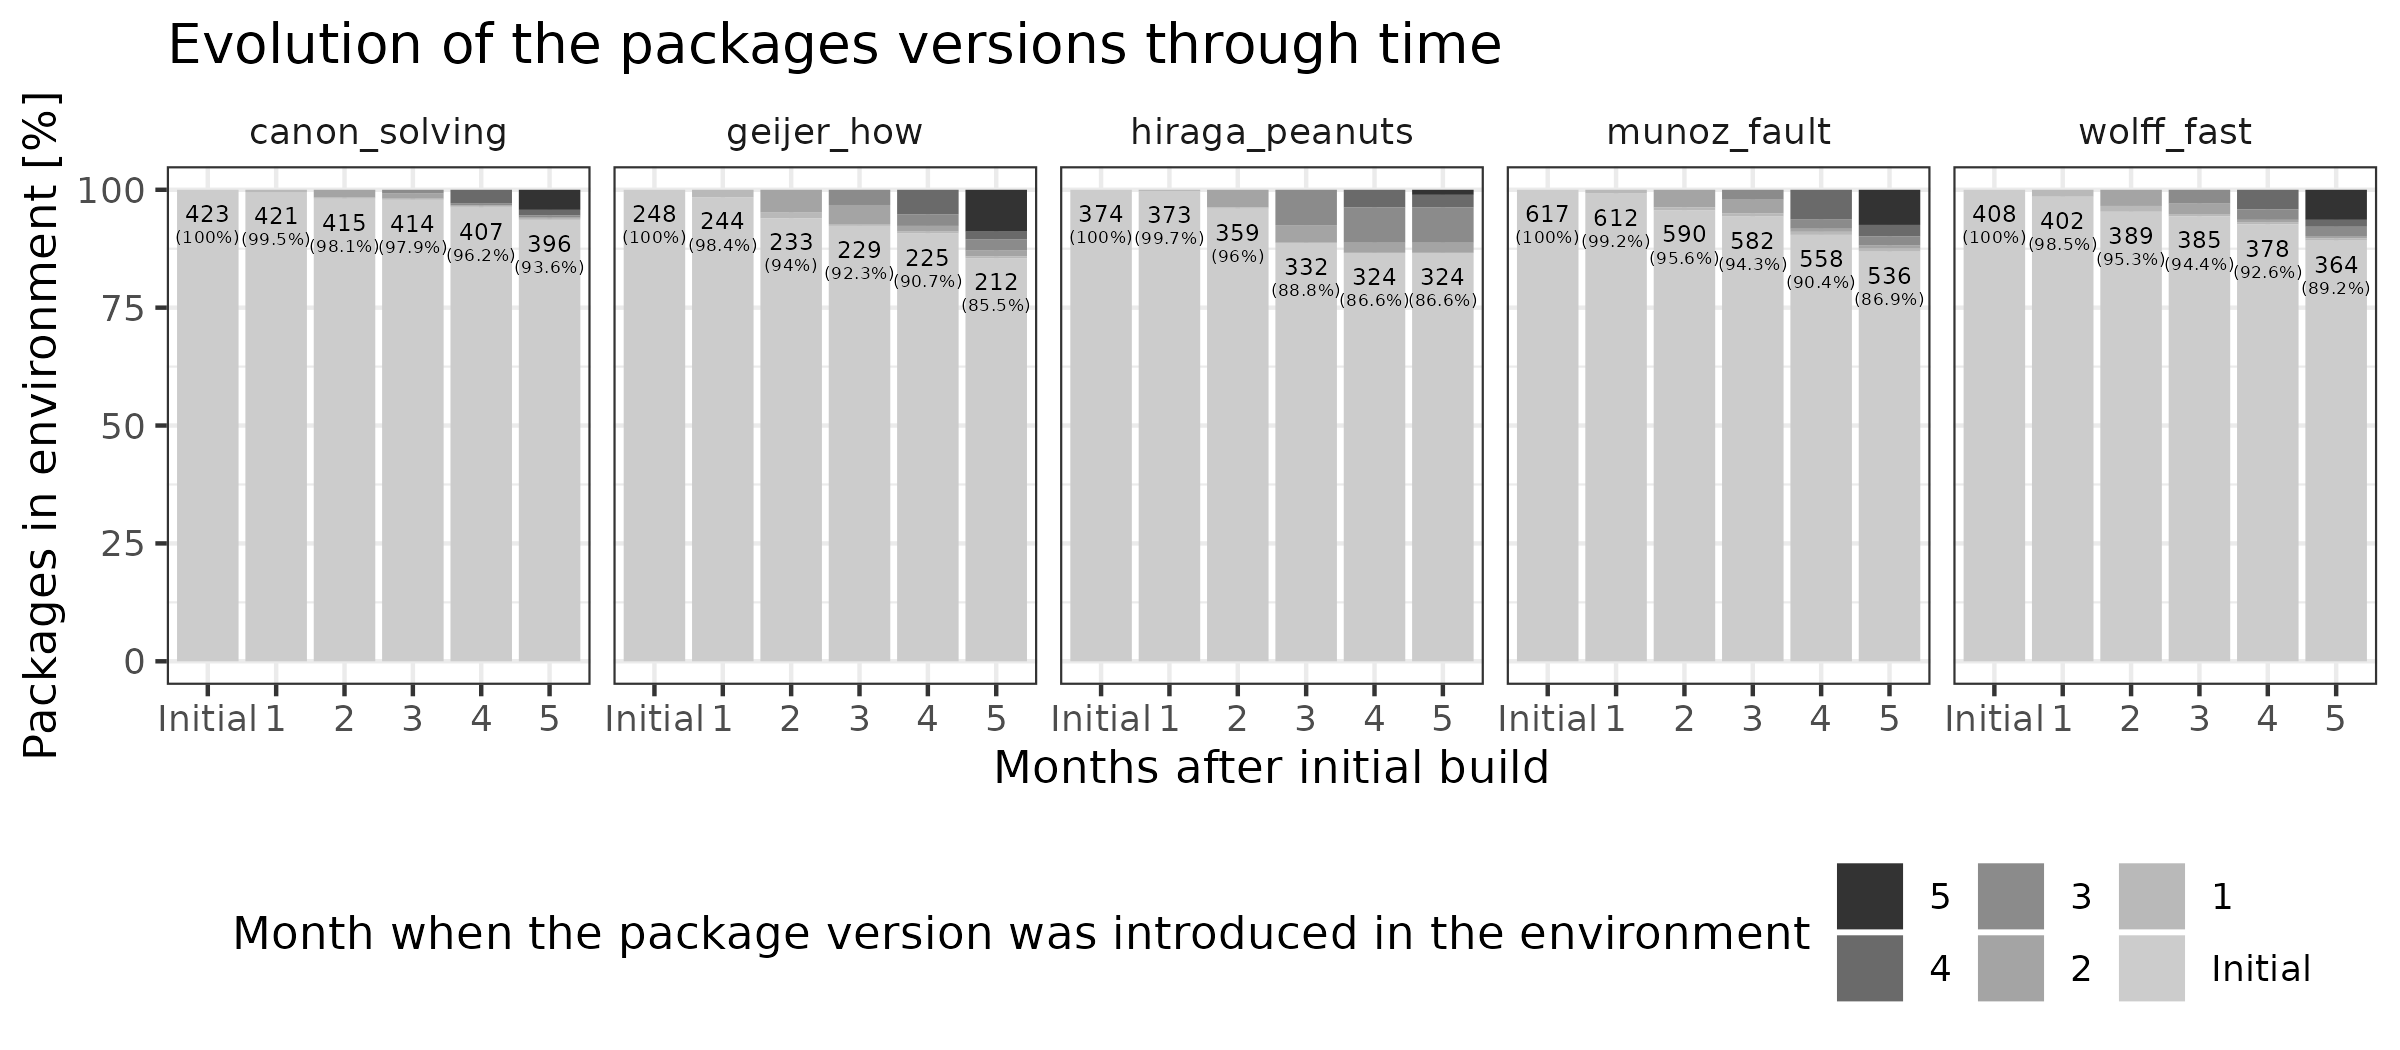
\includegraphics[width=\textwidth]{./fig.pdf}
  \caption{
    Evolution of the packages in the software environment of each container through time.
    Each container has been rebuilt once a month.
    The color of the bar corresponds to the month when a specific version of a package has been introduced in the software environment.
    We can see that the proportion of package versions similar to the versions in the initial build is decreasing throught the months.
  }
  \label{fig:results_per_artifact}
\end{figure*}

Figure~\ref{fig:results_per_artifact} depicts the evolution through time of the software environment produced by the \df\ of each studied artifact.
We can see that even after \emph{a single month} of the initial build, the software environment is already different for \emph{all} of the studied artifacts.
This is a severe threat to reproducibility as one month is the time-frame for a artifact evaluation process in conferences.
This means that the \df\ submitted by the authors can generate different software environment between the submission of the artifact and the reproduction attempt of the reviewers.

%\todo{a word on from ubuntu:latest and apt-get update}.

We can see that every month, new versions of packages are being introduced in the software environments of the containers.



\begin{figure}
  \centering
  \includegraphics[width=0.5\textwidth]{./fig2.pdf}
  \caption{
    plop
  }\label{fig:results_per_tool}
\end{figure}

Figure~\ref{fig:results_per_tool} depicts the evolution of the package version managed by each tool: \texttt{dpkg}, \texttt{git}, \texttt{pip} and manual download and build (\texttt{misc}).
We can see that the tools introducing variation in the software environment are \texttt{dpkg} and \texttt{pip}.

The packages that changed the most in terms of versions are:
\begin{enumerate}
\item \texttt{linux-libc-dev:amd64} (installed via \texttt{dpkg}) with 6 different versions for each artifact (1 per new build attempt)
\item \texttt{fonttools} (installed via \texttt{pip}) with 5 different versions for the artifacts \texttt{geijer\_how} and \texttt{wolff\_fast}
\item \texttt{numpy} (installed via \texttt{pip}) with 5 different versions for the artifact \texttt{wolff\_fast}
\end{enumerate}


% \newpage
\section{Conclusion and Perspectives}

% \subsection{Conclusion}
% 
% In this paper, we presented an initial version of \ecg, and its workflow, a tool to study the variations through time of containers from research artifacts.
% We evaluated the evolution of the software environment produced by \df\ from five artifacts from the EuroPar'24 conference.
% We observe that, even at this small scale, after only one month, there were variations in the produced software environments.
% Out of the popular tools to manage the software environment in a container, we have seen that \texttt{dpkg} and \texttt{pip} were the ones that introducing more undesired variations.
% 
% \df s are not solutions to capture on the \emph{long term} the software environment.
% There is a trade-off between storing the Docker images built by the authors and their recipe.
% Use Nix/Guix + Software Heritage.
% 
% Even if we only looked at \df s, this study could be extended to other technologies (Apptainer, virtual machines), but it was shown in \cite{guilloteau2024longevity} that \df s was the main solution to provided virtualized software environments.
% 
% In this paper, we presented the initial design of our framework to evaluate the longevity of the software environments generated with \df s from research artifacts.
% 
% We propose three possible scenarios for the longevity of the sharing of software environment:
% 
% \paragraph{Scenario 1: ``Business as usual''}
% Authors keep submitting non-reproducible \df s and conferences keep accepting them
% 
% \paragraph{Scenario 2: Storing everything forever}
% Authors store their version of the built container onto long-term storage (\eg\ Zenodo, Figshare), and artifact reviewers do not try to rebuild the \df\ but simply download the container.
% While this solution would allow the artifact reviewers and the future researchers to use the exact same software environment as the authors, it also raises \emph{sustainability questions}.
% Indeed, with the increase of scientific publications and the increase in artifact sharing in publications, can we community continue to store the built containers which ``weight'' orders of magnitude more than the recipe to generate them?
% Services such as Zenodo and Figshare are free, and backed up by public funding.
% Can these services run out of storage? or ask for a financial participation to archive data?
% 
% 
% \paragraph{Scenario 3: Change of practice}
% In this scenario, the community, \ie\ the conferences and the authors, change their practices related to reproducibility and software environment sharing.
% The community starts adopting solutions made for reproducibility of software environment (\ie\ Nix and Guix).
% Authors then simply have to share the recipe (text files) of their software environment for the artifact reviewers and future researchers to reproduce the results of their article.
% Moreover, Nix and Guix allow for the precise introduction of variation in the software environment, which is a crucial feature (not present in container technologies) in order to build upon previous artifact for future publications~\cite{mercier2018considering}.
% 
% 
% \subsection{Perspectives}
% 
% This paper aims to be an initial version of the design of a future larger study around the longevity of containers.
% We will thus write the descriptions of more artifact from more conferences, aiming for around a hundreds total containers, from conferences of various fields of Computer Science with various ``technical'' levels.
% 
% This initial work also raised more questions:
% \begin{itemize}
% \item Does the reduction of the proportion of package versions similar to the initial build will continue decreasing or will it eventually reach a ``stable state''? (for example 50\%)
% \item ...
% \end{itemize}

% -----------------------------------------------------------------

This paper presented the initial design of our longitudinal study of the evolution of the software environments produced by \df s.
We presented in Section \todo{ecg} \ecg, and its workflow (Section \todo{}), a tool to download, build and extract information from research artifacts \df.
Section \todo{protocole} presented the protocol to answer our scientific questions.
We showed initial results in Section \todo{expes} on five artifacts from the EuroPar'24 conference built every months for six months.
This initial study releaved that the software environments produced by the considered \df s variate \emph{every month} which highlights the lack of reproducibility of such practices.

A practice to deal with the lack of reproducibility of the \df s is for the authors to store the built container onto some long-time storage such as Zenodo.
However, this practice raises serious questions in terms of scalability and sustainability in terms of storage.
The lack of reproducibility of \df s shoud not be hidden with long-term storage: the practices from the conferences, journals, and the authors need to change.

%
% /////////////////////////////////////////////////////////////////////////////////////////////////////

\section*{Acknowledgments}

G5K, Antoine?

%% PAPER ENDS HERE -----------------------------------------------------------------------------------------------

\newpage
\newpage
%\bibliographystyle{sty/ACM-Reference-Format}
%\bibliography{references}
\printbibliography

\end{document}
